% Options for packages loaded elsewhere
\PassOptionsToPackage{unicode}{hyperref}
\PassOptionsToPackage{hyphens}{url}
%
\documentclass[
  man,floatsintext]{apa7}
\usepackage{amsmath,amssymb}
\usepackage{lmodern}
\usepackage{iftex}
\ifPDFTeX
  \usepackage[T1]{fontenc}
  \usepackage[utf8]{inputenc}
  \usepackage{textcomp} % provide euro and other symbols
\else % if luatex or xetex
  \usepackage{unicode-math}
  \defaultfontfeatures{Scale=MatchLowercase}
  \defaultfontfeatures[\rmfamily]{Ligatures=TeX,Scale=1}
\fi
% Use upquote if available, for straight quotes in verbatim environments
\IfFileExists{upquote.sty}{\usepackage{upquote}}{}
\IfFileExists{microtype.sty}{% use microtype if available
  \usepackage[]{microtype}
  \UseMicrotypeSet[protrusion]{basicmath} % disable protrusion for tt fonts
}{}
\makeatletter
\@ifundefined{KOMAClassName}{% if non-KOMA class
  \IfFileExists{parskip.sty}{%
    \usepackage{parskip}
  }{% else
    \setlength{\parindent}{0pt}
    \setlength{\parskip}{6pt plus 2pt minus 1pt}}
}{% if KOMA class
  \KOMAoptions{parskip=half}}
\makeatother
\usepackage{xcolor}
\usepackage{graphicx}
\makeatletter
\def\maxwidth{\ifdim\Gin@nat@width>\linewidth\linewidth\else\Gin@nat@width\fi}
\def\maxheight{\ifdim\Gin@nat@height>\textheight\textheight\else\Gin@nat@height\fi}
\makeatother
% Scale images if necessary, so that they will not overflow the page
% margins by default, and it is still possible to overwrite the defaults
% using explicit options in \includegraphics[width, height, ...]{}
\setkeys{Gin}{width=\maxwidth,height=\maxheight,keepaspectratio}
% Set default figure placement to htbp
\makeatletter
\def\fps@figure{htbp}
\makeatother
\setlength{\emergencystretch}{3em} % prevent overfull lines
\providecommand{\tightlist}{%
  \setlength{\itemsep}{0pt}\setlength{\parskip}{0pt}}
\setcounter{secnumdepth}{-\maxdimen} % remove section numbering
% Make \paragraph and \subparagraph free-standing
\ifx\paragraph\undefined\else
  \let\oldparagraph\paragraph
  \renewcommand{\paragraph}[1]{\oldparagraph{#1}\mbox{}}
\fi
\ifx\subparagraph\undefined\else
  \let\oldsubparagraph\subparagraph
  \renewcommand{\subparagraph}[1]{\oldsubparagraph{#1}\mbox{}}
\fi
\newlength{\cslhangindent}
\setlength{\cslhangindent}{1.5em}
\newlength{\csllabelwidth}
\setlength{\csllabelwidth}{3em}
\newlength{\cslentryspacingunit} % times entry-spacing
\setlength{\cslentryspacingunit}{\parskip}
\newenvironment{CSLReferences}[2] % #1 hanging-ident, #2 entry spacing
 {% don't indent paragraphs
  \setlength{\parindent}{0pt}
  % turn on hanging indent if param 1 is 1
  \ifodd #1
  \let\oldpar\par
  \def\par{\hangindent=\cslhangindent\oldpar}
  \fi
  % set entry spacing
  \setlength{\parskip}{#2\cslentryspacingunit}
 }%
 {}
\usepackage{calc}
\newcommand{\CSLBlock}[1]{#1\hfill\break}
\newcommand{\CSLLeftMargin}[1]{\parbox[t]{\csllabelwidth}{#1}}
\newcommand{\CSLRightInline}[1]{\parbox[t]{\linewidth - \csllabelwidth}{#1}\break}
\newcommand{\CSLIndent}[1]{\hspace{\cslhangindent}#1}
\ifLuaTeX
\usepackage[bidi=basic]{babel}
\else
\usepackage[bidi=default]{babel}
\fi
\babelprovide[main,import]{english}
% get rid of language-specific shorthands (see #6817):
\let\LanguageShortHands\languageshorthands
\def\languageshorthands#1{}
% Manuscript styling
\usepackage{upgreek}
\captionsetup{font=singlespacing,justification=justified}

% Table formatting
\usepackage{longtable}
\usepackage{lscape}
% \usepackage[counterclockwise]{rotating}   % Landscape page setup for large tables
\usepackage{multirow}		% Table styling
\usepackage{tabularx}		% Control Column width
\usepackage[flushleft]{threeparttable}	% Allows for three part tables with a specified notes section
\usepackage{threeparttablex}            % Lets threeparttable work with longtable

% Create new environments so endfloat can handle them
% \newenvironment{ltable}
%   {\begin{landscape}\centering\begin{threeparttable}}
%   {\end{threeparttable}\end{landscape}}
\newenvironment{lltable}{\begin{landscape}\centering\begin{ThreePartTable}}{\end{ThreePartTable}\end{landscape}}

% Enables adjusting longtable caption width to table width
% Solution found at http://golatex.de/longtable-mit-caption-so-breit-wie-die-tabelle-t15767.html
\makeatletter
\newcommand\LastLTentrywidth{1em}
\newlength\longtablewidth
\setlength{\longtablewidth}{1in}
\newcommand{\getlongtablewidth}{\begingroup \ifcsname LT@\roman{LT@tables}\endcsname \global\longtablewidth=0pt \renewcommand{\LT@entry}[2]{\global\advance\longtablewidth by ##2\relax\gdef\LastLTentrywidth{##2}}\@nameuse{LT@\roman{LT@tables}} \fi \endgroup}

% \setlength{\parindent}{0.5in}
% \setlength{\parskip}{0pt plus 0pt minus 0pt}

% Overwrite redefinition of paragraph and subparagraph by the default LaTeX template
% See https://github.com/crsh/papaja/issues/292
\makeatletter
\renewcommand{\paragraph}{\@startsection{paragraph}{4}{\parindent}%
  {0\baselineskip \@plus 0.2ex \@minus 0.2ex}%
  {-1em}%
  {\normalfont\normalsize\bfseries\itshape\typesectitle}}

\renewcommand{\subparagraph}[1]{\@startsection{subparagraph}{5}{1em}%
  {0\baselineskip \@plus 0.2ex \@minus 0.2ex}%
  {-\z@\relax}%
  {\normalfont\normalsize\itshape\hspace{\parindent}{#1}\textit{\addperi}}{\relax}}
\makeatother

% \usepackage{etoolbox}
\makeatletter
\patchcmd{\HyOrg@maketitle}
  {\section{\normalfont\normalsize\abstractname}}
  {\section*{\normalfont\normalsize\abstractname}}
  {}{\typeout{Failed to patch abstract.}}
\patchcmd{\HyOrg@maketitle}
  {\section{\protect\normalfont{\@title}}}
  {\section*{\protect\normalfont{\@title}}}
  {}{\typeout{Failed to patch title.}}
\makeatother

\usepackage{xpatch}
\makeatletter
\xapptocmd\appendix
  {\xapptocmd\section
    {\addcontentsline{toc}{section}{\appendixname\ifoneappendix\else~\theappendix\fi\\: #1}}
    {}{\InnerPatchFailed}%
  }
{}{\PatchFailed}
\keywords{keywords\newline\indent Word count: X}
\usepackage{csquotes}
\makeatletter
\renewcommand{\paragraph}{\@startsection{paragraph}{4}{\parindent}%
  {0\baselineskip \@plus 0.2ex \@minus 0.2ex}%
  {-1em}%
  {\normalfont\normalsize\bfseries\typesectitle}}
\renewcommand{\subparagraph}[1]{\@startsection{subparagraph}{5}{1em}%
  {0\baselineskip \@plus 0.2ex \@minus 0.2ex}%
  {-\z@\relax}%
  {\normalfont\normalsize\bfseries\itshape\hspace{\parindent}{#1}\textit{\addperi}}{\relax}}
\makeatother

\usepackage{tabu}
\usepackage{amsmath}
\usepackage{setspace}
\AtBeginEnvironment{tabular}{\singlespacing}
\AtBeginEnvironment{lltable}{\singlespacing}
\AtBeginEnvironment{tablenotes}{\doublespacing}
\captionsetup[table]{font={stretch=1.5}}
\captionsetup[figure]{font={stretch=1.5}}
\usepackage{float}
\floatplacement{figure}{H}
\usepackage[font=sf]{caption}
\usepackage[fontsize=11pt]{fontsize}
\newenvironment{fignote}{\begin{quote}\footnotesize}{\end{quote}}
\setlength{\textfloatsep}{0pt plus 1pt minus 1pt}
\newcommand{\squeezeup}{\vspace{-5mm}}
\usepackage{ragged2e}
\ifLuaTeX
  \usepackage{selnolig}  % disable illegal ligatures
\fi
\IfFileExists{bookmark.sty}{\usepackage{bookmark}}{\usepackage{hyperref}}
\IfFileExists{xurl.sty}{\usepackage{xurl}}{} % add URL line breaks if available
\urlstyle{same} % disable monospaced font for URLs
\hypersetup{
  pdftitle={Manipulating contextual cueing in real world scenes},
  pdfauthor={PsyBSc14 Grundlagen der Psychologie Vertiefung: Allgemeine Psycholgie I Jan Luca Schnatz Goethe University: Institut of Psychology Supervisor: M.Sc. Aylin Kallmayer Contact: s2787063@stud.uni-frankfurt.de November 2nd 2022},
  pdflang={en-EN},
  pdfkeywords={keywords},
  hidelinks,
  pdfcreator={LaTeX via pandoc}}

\title{Manipulating contextual cueing in real world scenes}
\author{PsyBSc14 Grundlagen der Psychologie Vertiefung: Allgemeine Psycholgie I \break Jan Luca Schnatz \break Goethe University: Institut of Psychology \break Supervisor: M.Sc. Aylin Kallmayer \break Contact: \href{mailto:s2787063@stud.uni-frankfurt.de}{\nolinkurl{s2787063@stud.uni-frankfurt.de}} \break November 2nd 2022\textsuperscript{}}
\date{}


\shorttitle{\phantom{test}}

\affiliation{\phantom{0}}

\abstract{%
One or two sentences providing a \textbf{basic introduction} to the field, comprehensible to a scientist in any discipline.

Two to three sentences of \textbf{more detailed background}, comprehensible to scientists in related disciplines.

One sentence clearly stating the \textbf{general problem} being addressed by this particular study.

One sentence summarizing the main result (with the words ``\textbf{here we show}'' or their equivalent).

Two or three sentences explaining what the \textbf{main result} reveals in direct comparison to what was thought to be the case previously, or how the main result adds to previous knowledge.

One or two sentences to put the results into a more \textbf{general context}.

Two or three sentences to provide a \textbf{broader perspective}, readily comprehensible to a scientist in any discipline.
}



\begin{document}
\maketitle

\hypertarget{introduction}{%
\section{Introduction}\label{introduction}}

Humans constantly exposed to an overloading flood of visual information competing for our attention, yet we are able to direct our attention precisely and quickly to targets that are relevant to us. This is rooted to a significant extent (this relies heavily) in the ability to harness the oftentimes stable and structured context of a scene by perceiving the invariant spatial arrangement between different objects in the environment and a target of interest. For example, if you search for your favourite psychology textbook in your tidy bookshelf, the book is located in a fixed location in relation to the familiar environment (i.e.~the other books), you are making you of this.The use of this contextual information in an invariant structure of the visual environment results in an increased predictability of the target location (i.e.~the spatial configuration of scene cues the location of the target), thus facilitating visual search (Chun, 2000).

Test citation: (Andersen, Müller, \& Martinovic, 2012)

(Mack \& Eckstein, 2011)

guidance
\newpage

\hypertarget{methods}{%
\section{Methods}\label{methods}}

\hypertarget{participants}{%
\subsection{Participants}\label{participants}}

\hypertarget{apparatus-and-stimulus-material}{%
\subsection{Apparatus and stimulus material}\label{apparatus-and-stimulus-material}}

\begin{figure}[H]

\begin{figure}

{\centering 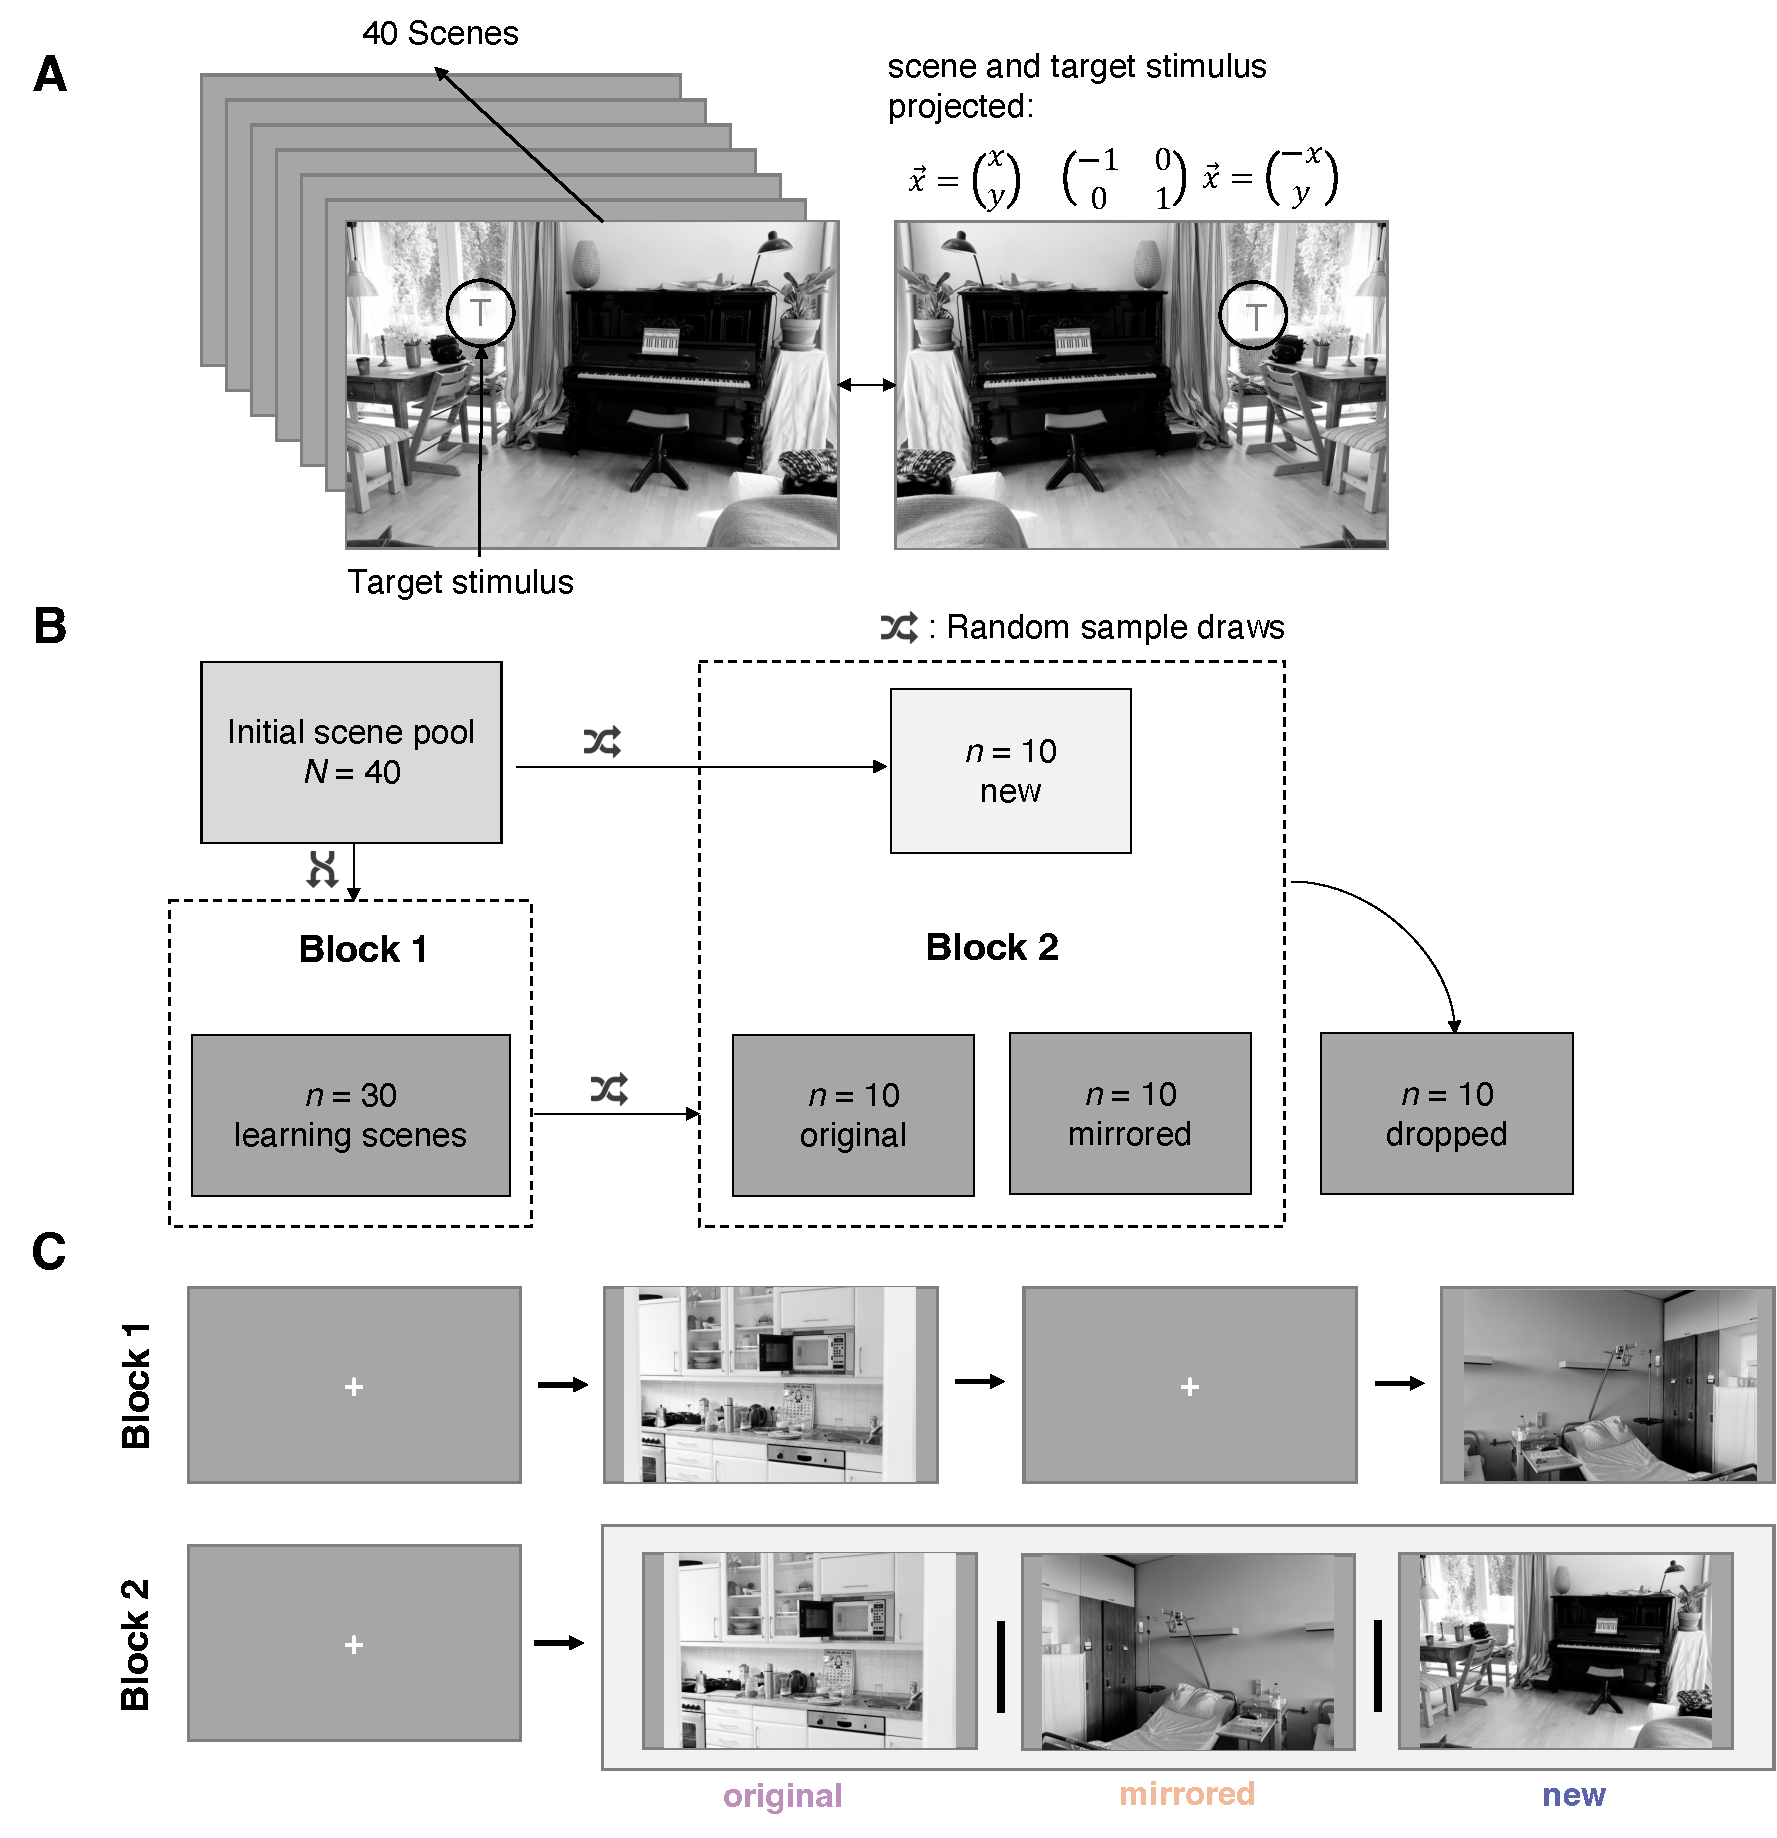
\includegraphics[width=0.8\linewidth]{../results/figures/experimental_design} 

}

\end{figure}

\caption{Experimental design and procedure\label{fig:experimental-design}}
\begingroup
\footnotesize
\textit{Note:} \textbf{A}. 40 scenes of the BoIS dataset (Mohr et al., 2016) were chosen as the stimulus pool for the experiment. Participants were required to search a target stimulus (T) in each presented scene. For mirrored scenes in the second block, the target stimulus was also projected along the horizontal axis.  \textbf{B}. From the initial 40 scenes, 30 scenes were randomly sampled for each participant in block 1. Subsequently, from these sampled scenes,  10 scenes were presented unmirrored (original) and mirrored respectively. To allow a baseline comparison, 10 new scenes that were not shown to the participants berfore, were included in block 2. \textbf{C}. All trial sequences started the presentation of a fixation cross and then proceeded in the aforementioned procedure. 
\endgroup
\end{figure}

\hypertarget{trial-sequence}{%
\subsection{Trial sequence}\label{trial-sequence}}

\hypertarget{design-and-procedure}{%
\subsection{Design and procedure}\label{design-and-procedure}}

\hypertarget{data-analysis}{%
\subsection{Data analysis}\label{data-analysis}}

\hypertarget{results}{%
\section{Results}\label{results}}

\hypertarget{data-transformation}{%
\subsection{Data transformation}\label{data-transformation}}

\hypertarget{descriptive-results}{%
\subsection{Descriptive results}\label{descriptive-results}}

\hypertarget{lmm-results}{%
\subsection{LMM results}\label{lmm-results}}

\hypertarget{further-analysis}{%
\subsection{Further analysis}\label{further-analysis}}

\newpage

\begin{figure}[H]

\begin{figure}

{\centering 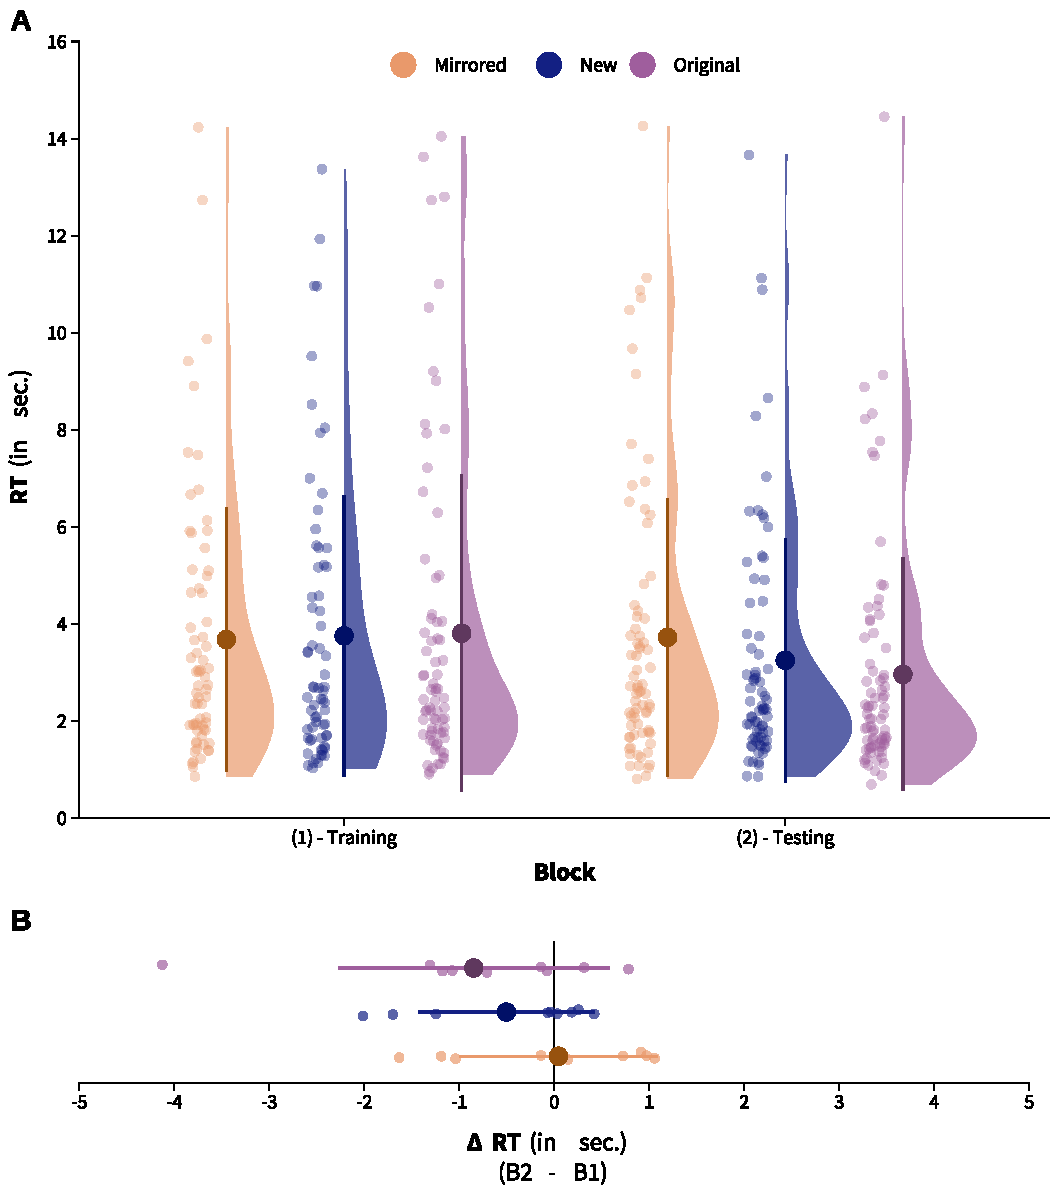
\includegraphics[width=0.8\linewidth]{../results/figures/combined_rt_diff} 

}

\end{figure}

\caption{Descriptive reaction time differences between the learning and testing block for each condition (new, original and mirrored)
\label{fig:rt-diff}}
\begingroup
\footnotesize
\textit{Note:} \textbf{A}. Figure displays the density distributions for each level of the two conditions block and orientation, as well as the jittered raw data points. The pointrange indicates the mean reaction time (RT) in each condition as well as the lower and upper SEM. \textbf{B}. Figure displays the aggregated reaction time differences between block 2 and block 1 (B2 - B1) for each participant. Negative values consequently indicate, that the reaction time was lower in block 2 compared to block 1.
\endgroup
\end{figure}

\begin{singlespace}
\begingroup\fontsize{10}{12}\selectfont

\begin{ThreePartTable}
\begin{TableNotes}[para]
\item \textit{Note.} 
\item $n$: total number of hits in each condition, $M$: mean, $SD$: standard deviation.
\end{TableNotes}
\begin{longtabu} to \linewidth {>{\raggedright}X>{\centering}X>{\centering}X>{\centering}X>{\centering}X>{\centering}X>{\centering}X}
\caption{\label{tab:unnamed-chunk-1}Descriptive table of the the reaction times and hit rates for each level of the two factors block and orientation}\\
\toprule
\multicolumn{1}{c}{ } & \multicolumn{3}{c}{Block 1} & \multicolumn{3}{c}{Block 2} \\
\cmidrule(l{3pt}r{3pt}){2-4} \cmidrule(l{3pt}r{3pt}){5-7}
\multicolumn{1}{c}{Orientation} & \multicolumn{1}{c}{$M$ ($SD$)} & \multicolumn{1}{c}{$n$} & \multicolumn{1}{c}{Hit rate} & \multicolumn{1}{c}{$M$  ($SD$) } & \multicolumn{1}{c}{$n$ } & \multicolumn{1}{c}{Hit rate }\\
\midrule
Original & 3.81 (3.27) & 74 & 0.82 & 2.96 (2.4) & 78 & 0.87\\
Mirrored & 3.68 (2.72) & 69 & 0.77 & 3.73 (2.87) & 75 & 0.83\\
New & 3.76 (2.9) & 67 & 0.74 & 3.25 (2.52) & 75 & 0.83\\
\bottomrule
\insertTableNotes
\end{longtabu}
\end{ThreePartTable}
\endgroup{}
\end{singlespace}

\begin{singlespace}
\begingroup\fontsize{10}{12}\selectfont

\begin{ThreePartTable}
\begin{TableNotes}[para]
\item \textit{Note.} 
\item Significance was obtained using parametric bootstrapping with n = 5000 resamples. If the 95 confidence interval (CI) encompasses zero, the regression weight is statistically non-significant. Because all predictors are discrete variables, treatment contrast coding was used (baseline for factor block: block 1, reference level for factor orientation: new condition) : contrast coded regression weight of the block
\end{TableNotes}
\begin{longtabu} to \linewidth {>{\raggedright}X>{\centering}X>{\centering}X>{\centering}X>{\centering}X>{\centering}X}
\caption{\label{tab:unnamed-chunk-2}Summary of the linear mixed model results for the fixed effects of block and orientation as well as crossed random effects for participant and scene}\\
\toprule
\multicolumn{1}{c}{Term} & \multicolumn{1}{c}{$\hat{\beta}$ / $\sigma^{2}$} & \multicolumn{1}{c}{\textit{SE}} & \multicolumn{1}{c}{\textit{t}} & \multicolumn{1}{c}{95\% CI} & \multicolumn{1}{c}{Significance}\\
\midrule
\addlinespace[0.3em]
\multicolumn{6}{l}{Fixed}\\
\hspace{1em}Intercept $\beta_{0}$ & 0.837 & 0.068 & 12.244 & {}[0.702, 0.971] & $\ast$\\
\hspace{1em}Block $\beta_{1}$ & -0.018 & 0.066 & -0.265 & {}[-0.148, 0.114] & n.s.\\
\hspace{1em}Orient. $\beta_{2}$ & 0.005 & 0.07 & 0.074 & {}[-0.132, 0.145] & n.s.\\
\hspace{1em}Orient. $\beta_{3}$ & -0.02 & 0.068 & -0.295 & {}[-0.157, 0.114] & n.s.\\
\hspace{1em}Int. $\beta_{4}$ & -0.058 & 0.095 & -0.609 & {}[-0.251, 0.122] & n.s.\\
\hspace{1em}Int. $\beta_{5}$ & -0.107 & 0.093 & -1.157 & {}[-0.29, 0.072] & n.s.\\
\addlinespace[0.3em]
\multicolumn{6}{l}{Random}\\
\hspace{1em}$\sigma^{2}_{scene}$ & 0.01 & - & - & - & -\\
\hspace{1em}$\sigma^{2}_{participant}$ & 0.018 & - & - & - & -\\
\hspace{1em}$\sigma^{2}_{\epsilon}$ & 0.158 & - & - & - & -\\
\bottomrule
\insertTableNotes
\end{longtabu}
\end{ThreePartTable}
\endgroup{}
\end{singlespace}

\begin{equation}
\begin{gathered}
y_{ijk} = \gamma_{00} + v_{0k} + u_{0j} + 
\beta_1~E_{ijk}+ \beta_2~O_{1_{ijk}}~ \beta_3~O_{2_{ijk}} + \\
\beta_4 ~ (E_{ijk}~O_{1_{ijk}}) + \beta_5~(E_{ijk} ~O_{2_{ijk}}) +  
\epsilon_{ijk}
\end{gathered}
\end{equation}

\[\epsilon_{ijk} \sim \mathcal{N}(0, \sigma^2),~~ u_{0k} \sim \mathcal{N}(0, \sigma^2_{u_{0k}}),~~ u_{0j} \sim \mathcal{N}(0, \sigma^2_{u_{0j}})\]

\hypertarget{discussion}{%
\section{Discussion}\label{discussion}}

\newpage

\hypertarget{references}{%
\section{References}\label{references}}

\hypertarget{refs}{}
\begin{CSLReferences}{1}{0}
\leavevmode\vadjust pre{\hypertarget{ref-andersen_bottom-up_2012}{}}%
Andersen, S., Müller, M., \& Martinovic, J. (2012). Bottom-{Up} {Biases} in {Feature}-{Selective} {Attention}. \emph{The Journal of Neuroscience : The Official Journal of the Society for Neuroscience}, \emph{32}, 16953--16958. \url{https://doi.org/10.1523/JNEUROSCI.1767-12.2012}

\leavevmode\vadjust pre{\hypertarget{ref-chun_contextual_2000}{}}%
Chun, M. M. (2000). Contextual cueing of visual attention. \emph{Trends in Cognitive Sciences}, \emph{4}(5), 170--178. \url{https://doi.org/10.1016/S1364-6613(00)01476-5}

\leavevmode\vadjust pre{\hypertarget{ref-mack_object_2011}{}}%
Mack, S. C., \& Eckstein, M. P. (2011). Object co-occurrence serves as a contextual cue to guide and facilitate visual search in a natural viewing environment. \emph{Journal of Vision}, \emph{11}(9), 9--9. \url{https://doi.org/10.1167/11.9.9}

\end{CSLReferences}

\newpage

\hypertarget{appendix-appendix}{%
\appendix}


\begin{singlespace}
\begingroup\fontsize{10}{12}\selectfont

\begin{ThreePartTable}
\begin{TableNotes}[para]
\item \textit{Note.} 
\item This is a test.
\end{TableNotes}
\begin{longtabu} to \linewidth {>{\raggedright}X>{\centering}X>{\centering}X>{\centering}X}
\caption{\label{tab:unnamed-chunk-4}Transformation Statistics}\\
\toprule
\multicolumn{1}{c}{Transformation} & \multicolumn{1}{c}{$M$ ($SD$)} & \multicolumn{1}{c}{$\lambda$} & \multicolumn{1}{c}{$\chi^2$ / $df$}\\
\midrule
Box-Cox & 0.79 (0.43) & -0.39 & 1.12\\
Yeo-Johnson & 0.79 (0.15) & -0.83 & 1.21\\
$log_{10}(x)$ & 0.44 (0.29) & - & 1.53\\
$arcsinh(x)$ & 1.77 (0.62) & - & 1.95\\
$\sqrt{x}$ & 1.76 (0.64) & - & 3.05\\
\addlinespace
no transformation & 3.52 (2.79) & - & 6.22\\
$e^x$ & 2.388342e+04 (1.647217e+05) & - & 46.52\\
\bottomrule
\insertTableNotes
\end{longtabu}
\end{ThreePartTable}
\endgroup{}
\end{singlespace}

\begin{singlespace}
\begingroup\fontsize{10}{12}\selectfont

\begin{ThreePartTable}
\begin{TableNotes}[para]
\item \textit{Note.} 
\item This is a test
\end{TableNotes}
\begin{longtabu} to \linewidth {>{\raggedright}X>{\centering}X>{\centering}X}
\caption{\label{tab:unnamed-chunk-5}ANOVA comparison table}\\
\toprule
\multicolumn{1}{c}{Measures of fit} & \multicolumn{1}{c}{(1)} & \multicolumn{1}{c}{(2)}\\
\midrule
$AIC$ & 483.524 & 466.043\\
$BIC$ & 520.264 & 510.948\\
L($\theta$) & -232.762 & -222.022\\
Deviance & 465.524 & 444.043\\
$t$ & - & 21.481\\
\addlinespace
$df$ & - & 2\\
$p$ & - & < .001\\
\bottomrule
\insertTableNotes
\end{longtabu}
\end{ThreePartTable}
\endgroup{}
\end{singlespace}

\begin{figure}[H]

\begin{figure}
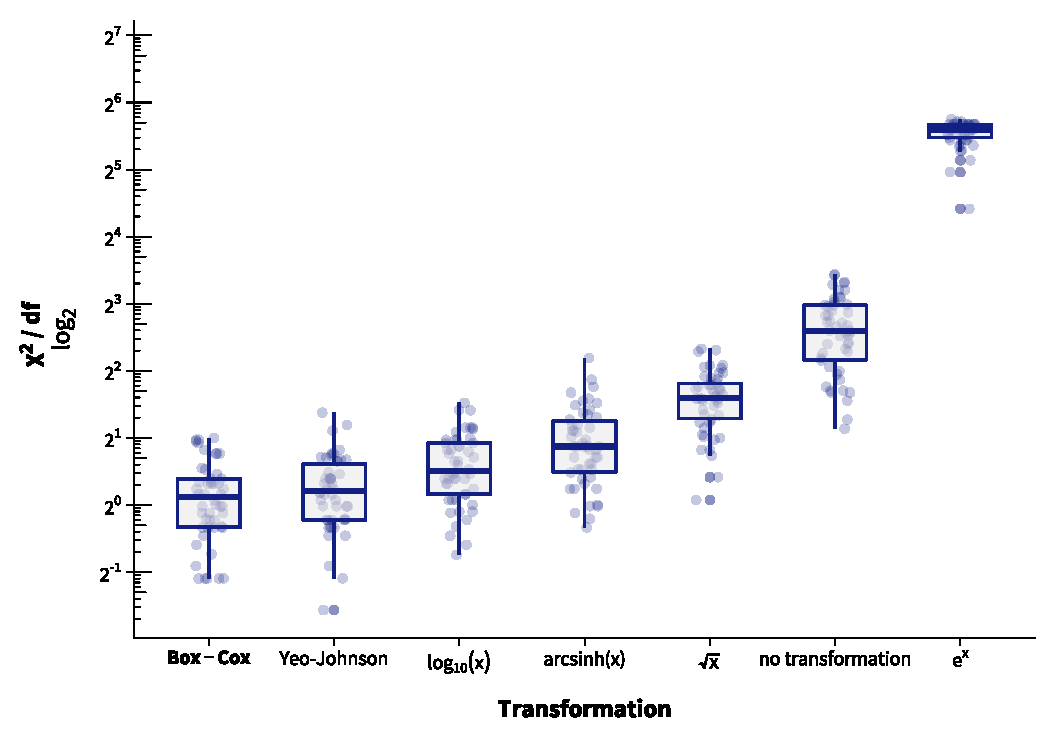
\includegraphics[width=0.9\linewidth]{../results/figures/rt_transformation} \end{figure}

\caption{Performance comparison between different transformation methods to approximate a normal distribution. \label{fig:pressure}}
\begingroup
\footnotesize
\textit{Notes:} $\chi^2$ / $df$ is the Pearson normality statistic divided by its degrees of freedom. Lower values indicates better normality fit. Ordinate is displayed on a $log_2$ scale to enhance visibility.
\endgroup
\end{figure}


\end{document}
